\section{Вступ}
\label{sec:intro}

За мету в цій лабораторній роботі я ставив собі попрацювати і набути практичних навичок зі смарт-контрактами Ethereum 
(у продовження першої лаби). У Завданні 1 я візьму один з еталонних контрактів з офіційної документації Solidity (версія~0.5.3, «Solidity by Example»), 
розгорну його в тестовій мережі Sepolia та спробую покращити його газову ефективність. А потім ще спробую накняпати ще контракт 
власними силами (а-ля завдання 2).

На \href{https://docs.soliditylang.org/en/v0.5.3/solidity-by-example.html}{сайті Solidity}~\cite{solidity-docs} наведено такі приклади контрактів:

\begin{enumerate}[label=\arabic*.]
    \item \textbf{Voting (Ballot)} --- система делегованого голосування з контролем доступу.
    \item \textbf{Simple Auction} --- відкритий аукціон з ефірним депозитом.
    \item \textbf{Blind Auction} --- аукціон з розкриттям ставок після їхнього підтвердження з хешованими ставками.
    \item \textbf{Payment Channel} --- позаланцюгові мікроплатежі з підписами.
\end{enumerate}

Зупинюся я на контракті \textbf{Ballot (Voting)} (Голосування), оскільки він демонструє найширший спектр можливостей 
мови Solidity~\cite{solidity-lang} -- структури, відображення, контроль доступу, логіку делегування та функції перегляду, і при цьому не вимагає 
переказів Ether, що спрощує тестування. Крім того, його механізм делегування містить чітку можливість оптимізації газу 
(необмежений цикл \texttt{while}).

\section{Як працюють смарт-контракти (in general)}
\label{sec:general}

\subsection{Визначення}

\emph{Smart contract} це певна програма, що зберігається в блокчейні Ethereum і виконується автоматично при виклику 
її функцій. Життєвий цикл складається з чотирьох етапів:

\begin{enumerate}[label=\textbf{\arabic*.}]
    \item \textbf{Writing.} Розробник пише вихідний код у Solidity (\texttt{.sol}). Компілятор (\texttt{solc}) створює два артефакти:
        \begin{itemize}
            \item \emph{EVM bytecode} --- низькорівневі інструкції, що виконуються віртуальною машиною Ethereum.
            \item \emph{ABI (Application Binary Interface)} --- опис у форматі JSON усіх публічних функцій, їхніх параметрів 
                та типів повернення. Зовнішні інструменти, такі як (web3.js, ethers.js, Remix), використовують ABI для кодування/декодування 
                викликів.
        \end{itemize}
    \item \textbf{Deployment.} Спеціальна транзакція з порожнім полем \texttt{to} надсилає байт-код до мережі. 
        EVM виконує \texttt{constructor()} рівно один раз, ініціалізує змінні стану, а мережа присвоює 
        контракту постійну адресу.
    \item \textbf{Interaction.} Користувачі (або інші контракти) викликають функції одним із двох способів:
        \begin{itemize}
            \item \emph{State-changing functions} (write) --- створюють транзакцію, яка має бути підтверджена в блокчейні; (cost gas).
            \item \emph{View / pure functions} (read) --- виконується локально by node, (free of charge).
        \end{itemize}
    \item \textbf{Termination.} Контракт існує в ланцюжку безстроково. Його можна зробити нефункціональним за допомогою 
        операційного коду \texttt{selfdestruct} (застарілого в сучасній Solidity) або шляхом впровадження шаблону паузи/знищення.
\end{enumerate}

\subsection{Стан, газ і вартість контрактів (EVM Storage and Gas)}

Стан контракту зберігається в постійній пам'яті (\emph{storage slots}), кожен з яких має ширину 256 біт. Запис у новий слот коштує 20000~gas (\texttt{SSTORE}); 
оновлення існуючого слота коштуватиме 5 000 газу; читання коштує 2 100 газу (\texttt{SLOAD}). Пам'ять (тимчасова, для кожного виклику) і дані 
виклику (тільки для читання, для аргументів функції) значно дешевші~\cite{solidity-gas}.

Кожен виконуваний EVM код має фіксовану газову вартість. Відправник транзакції вказує \emph{gas limit}, а також сплачує $\text{gas used} \times \text{gas price}$ в ETH. 
Якщо газ закінчується в процесі виконання, всі зміни стану скасовуються, і (що важливо!) спожитий газ на рахунок \emph{не} повертається. 
Цей механізм запобігає нескінченним циклам і стимулює писати ефективний код.

\subsection{Події (Events)}

Контракти можуть \texttt{emit} (продукувати) певні події. Ці події зберігаються в ланцюжку як журнали транзакцій (це набагато дешевше, 
ніж зберігання: $\sim$375~gas base + 375~gas per indexed topic + 8~gas per byte of data). Вони доступні для запиту поза ланцюжком, але 
\emph{не} доступні для читання іншими контрактами.

\subsection{Діаграма життєвого циклу смарт-контракту}

\begin{figure}[H]
    \centering
    \begin{tikzpicture}[
        node distance=1.8cm,
        every node/.style={font=\small},
        block/.style={
            rectangle, draw, rounded corners=4pt,
            minimum width=3.5cm, minimum height=1cm,
            fill=blue!8, align=center
        },
        arr/.style={-{Stealth[length=3mm]}, thick}
    ]
        \node[block] (write) {1. Writing\\(\texttt{.sol} source)};
        \node[block, right=of write] (compile) {Compilation\\(bytecode + ABI)};
        \node[block, right=of compile] (deploy) {2. Deployment\\(constructor tx)};
        \node[block, below=of deploy] (chain) {On-chain\\contract address};
        \node[block, left=of chain] (interact) {3. Interaction\\(call / send tx)};
        \node[block, left=of interact] (state) {State changes\\or view results};

        \draw[arr] (write) -- (compile);
        \draw[arr] (compile) -- (deploy);
        \draw[arr] (deploy) -- (chain);
        \draw[arr] (chain) -- (interact);
        \draw[arr] (interact) -- (state);
    \end{tikzpicture}
    \caption{Smart contract lifecycle on Ethereum.}
    \label{fig:lifecycle}
\end{figure}

\section{Ballot Contract}
\label{sec:ballot}

Даний розділ я хочу присвятити детальному огляну оригінального контракту \texttt{Ballot} з офіційної документації Solidity 0.5.3, включаючи 
його структури даних, змінні стану та функції.

\subsection{Призначення договору}

Контракт Ballot реалізує \emph{delegated voting} (делеговане голосування). Головуючий створює бюлетень із переліком пропозицій. Він надає право голосу 
окремим адресам. Кожен уповноважений виборець може або проголосувати безпосередньо за пропозицію, або делегувати (передати) свій голос 
іншому виборцю, якому він довіряє. В кінці будь-хто може дізнатися, яка пропозиція перемогла.

\subsection{Структури даних}

\newpage
\subsubsection{\texttt{struct Proposal} (пропозиція)}

\begin{minted}{solidity}
    struct Proposal {
        bytes32 name;     // Short name (up to 32 bytes)
        uint voteCount;   // Accumulated votes
    }
\end{minted}

Тут використовується тип \texttt{bytes32} замість \texttt{string}, оскільки він займає рівно один 256-бітний слот пам'яті, тоді як \texttt{string} вимагає динамічного розподілу пам'яті і є значно дорожчим у газовому вираженні.

\subsubsection{\texttt{struct Voter}}

\begin{minted}{solidity}
    struct Voter {
        uint weight;      // Voting power (0 = no right, 1+ = can vote)
        bool voted;       // True after voting or delegating
        address delegate; // Delegation target; address(0) if none
        uint vote;        // Index of chosen proposal (meaningful only
                          //   if voted==true && delegate==address(0))
    }
\end{minted}

\begin{table}[H]
    \begin{tblr}{
            colspec = {Q[font=\ttfamily, l, m] X[l, m]},
            row{1} = {font=\bfseries, c},
            hlines, vlines,
            measure = vbox,
            width = \textwidth,
        }
        Поле     & Опис                                                                                                                                                                                            \\
        weight   & Право голосу. Ініціалізується 0 для всіх адрес. Встановлюється 1 головуючим за допомогою функції \texttt{giveRightToVote()}. Збільшується, коли інші виборці делегують право голосу цій адресі. \\
        voted    & Boolean flag. Встановлюється на \texttt{true} як у випадку, коли виборець голосує сам \emph{або} коли він делегує свої повноваження. Запобігає подвійному голосуванню.                          \\
        delegate & Адреса Ethereum, якій виборець делегував свої повноваження. Залишається 0, якщо виборець проголосував самостійно або ще не вчинив жодних дій                                                    \\
        vote     & Index в масиві \texttt{proposals[]}. Використовується лише тоді, коли виборець голосує безпосередньо (не делегує).                                                                              \\
    \end{tblr}
\end{table}

\subsection{Станові змінні}

\begin{minted}{solidity}
    address public chairperson;
    mapping(address => Voter) public voters;
    Proposal[] public proposals;
\end{minted}

\begin{table}[H]
    \begin{tblr}{
        colspec = {Q[font=\ttfamily, l, m]Q[font=\ttfamily, l, m]X[l, m]},
        row{1} = {font=\bfseries},
        hlines, vlines,
        width = \textwidth,
        }
        Змінна      & Тип        & Призначення                                                                        \\
        chairperson & address    & Зберігає адресу розробника контракту. Тільки ця адреса може надавати право голосу. \\
        voters      & mapping    & Відображає кожну адресу Ethereum у структуру \texttt{Voter}.                       \\
        proposals   & Proposal[] & Динамічний масив всіх пропозицій. Створюється конструктором один раз.              \\
    \end{tblr}
\end{table}

\begin{remark}
    Відображення не зберігає ключі, тому неможливо пройти по всіх виборцях в ланцюжку.
\end{remark}

\subsection{Конструктор}

\begin{minted}{solidity}
    constructor(bytes32[] memory proposalNames) public {
        chairperson = msg.sender;
        voters[chairperson].weight = 1;

        for (uint i = 0; i < proposalNames.length; i++) {
            proposals.push(Proposal({
                name: proposalNames[i],
                voteCount: 0
            }));
        }
    }
\end{minted}

Конструктор виконується \emph{exactly once} під час розгортання контракту. Він записує \texttt{msg.sender} як головуючого, автоматично надає йому 
вагу голосу ~1 і заповнює масив \texttt{proposals} з наданих йому імен. Вартість газу для розгортання пропорційна 
кількості пропозицій (кожен \texttt{push} записує новий слот пам'яті).

\subsection{Функція: \texttt{giveRightToVote(address voter)}}

\begin{minted}{solidity}
    function giveRightToVote(address voter) public {
        require(msg.sender == chairperson,
                "Only chairperson can give right to vote.");
        require(!voters[voter].voted,
                "The voter already voted.");
        require(voters[voter].weight == 0);
        voters[voter].weight = 1;
    }
\end{minted}

\noindent Функція застосовує три заходи безпеки:
\begin{enumerate}
    \item Тільки головуючий може її викликати (access control).
    \item Цільова адреса must not already possess voting rights (я хз як це перекласти нормально).
    \item Ціль не повинна ще мати права голосу (\texttt{weight == 0}).
\end{enumerate}

У разі успіху вага виборця встановлюється на ~1, що дозволяє йому брати участь у голосування. Приблизна вартість газу складає: 
$\sim$47\,000 (запис нового слота пам'яті).

\textbf{Обмеження:} Кожен виборець потребує окремої транзакції. Для $N$ виборців головуючий сплачує $N \times (\sim\!47\,000 + 21\,000_{\text{base}})$ газу. 
У самій документації Solidity розробники ставлять нам питання: \emph{"Чи можете ви придумати кращий спосіб?"{}} -- на це питання я дам в розділі з оптимізацією.

\subsection{Функція: \texttt{delegate(address to)}}

Це, певно, найскладніша функція в контракті. Виглядає вона наступним чином:

\newpage
\begin{minted}{solidity}
    function delegate(address to) public {
        Voter storage sender = voters[msg.sender];
        require(!sender.voted, "You already voted.");
        require(to != msg.sender, "Self-delegation is disallowed.");

        while (voters[to].delegate != address(0)) {
            to = voters[to].delegate;
            require(to != msg.sender, "Found loop in delegation.");
        }

        sender.voted = true;
        sender.delegate = to;
        Voter storage delegate_ = voters[to];

        if (delegate_.voted) {
            proposals[delegate_.vote].voteCount += sender.weight;
        } else {
            delegate_.weight += sender.weight;
        }
    }
\end{minted}

\begin{enumerate}
    \item Завантажує структуру \texttt{Voter} виборця за посиланням (\texttt{storage} pointer).
    \item Перевіряє, що виборець ще не голосував і не делегує сам собі.
    \item \textbf{Розв'язує ланцюжок делегування:} Цикл \texttt{while} проходить ланцюг делегування (A$\to$B$\to$C) 
        до тих пір, поки не знайде виборця, який не делегує далі. Цей цикл також перевіряє наявність циклічного делегування.
    \item Позначає виборця як проголосовавшого та записує остаточного делегата.
    \item \textbf{Два результати:}
    \begin{itemize}
        \item Якщо остаточний делегат вже голосував, вага виборця додається безпосередньо до обраної ним пропозиції.
        \item Якщо остаточний делегат ще не голосував, вага виборця переноситься до делегата (накопичуючи voting power).
    \end{itemize}
\end{enumerate}

\noindent \textbf{газові ризики:} Цикл \texttt{while} зчитує storage, сплачуючи (\texttt{SLOAD} = 2\,100~gas) на кожній ітерації. 
Ланцюжок делегування довжиною $k$ коштує приблизно $k \times 2\,100$~gas лише за один цикл. Чим довше ланцюжок, тим 
більша ймовірність вичерпати газовий ліміт блоку.

\subsection{Функція: \texttt{vote(uint proposal)}}

\begin{minted}{solidity}
    function vote(uint proposal) public {
        Voter storage sender = voters[msg.sender];
        require(sender.weight != 0, "Has no right to vote");
        require(!sender.voted, "Already voted.");

        sender.voted = true;
        sender.vote = proposal;
        proposals[proposal].voteCount += sender.weight;
    }
\end{minted}

Все доволі просто: позначити виборця як проголосовавшого, записати його вибір і додати його вагу до підрахунку обраної пропозиції. 
Якщо індекс \texttt{proposal} виходить за межі масиву, Solidity автоматично викликає \texttt{revert}, скасовуючи всі зміни стану. 
Вартість по газу: $\sim$47\,000--65\,000 залежно від того, чи слоти пам'яті є новими або вже записаними.

\subsection{Функції перегляду: \texttt{winningProposal()} and \texttt{winnerName()}}

\begin{minted}{solidity}
    function winningProposal() public view
        returns (uint winningProposal_)
    {
        uint winningVoteCount = 0;
        for (uint p = 0; p < proposals.length; p++) {
            if (proposals[p].voteCount > winningVoteCount) {
                winningVoteCount = proposals[p].voteCount;
                winningProposal_ = p;
            }
        }
    }

    function winnerName() public view
        returns (bytes32 winnerName_)
    {
        winnerName_ = proposals[winningProposal()].name;
    }
\end{minted}

Обидві функції є типу \texttt{view}. Це означає, що вони не змінюють стан і \emph{free to call} (без транзакції, без витрати газу) 
ззовні. Функція \texttt{winningProposal()} ітерує по всіх пропозиціях та повертає індекс тієї, яка має найбільшу кількість 
голосів (\texttt{voteCount}). Функція \texttt{winnerName()} викликає вищезгадану для отримання індексу переможця, а потім просто 
повертає його ім'я.

\textbf{Обмеження:} Не враховує рівність голосів! Якщо є випадок, де дві пропозиції мають однакову кількість голосів, перемогу отримує та, яка має нижчий індекс.

\subsection{Діаграма взаємодії контрактів}

Візуалізувати це можна наступним чином:

\begin{figure}[H]
    \centering
    \begin{tikzpicture}[
        node distance=1.4cm and 2.5cm,
        every node/.style={font=\small},
        actor/.style={
            rectangle, draw, rounded corners=3pt,
            minimum width=2.8cm, minimum height=0.9cm,
            fill=orange!15, align=center
        },
        func/.style={
            rectangle, draw, rounded corners=3pt,
            minimum width=3.2cm, minimum height=0.9cm,
            fill=green!10, align=center
        },
        arr/.style={-{Stealth[length=2.5mm]}, thick, draw=gray!70}
    ]
        % Actors
        \node[actor] (chair) {Chairperson};
        \node[actor, below=3.0cm of chair] (voter) {Voter};

        % Functions
        \node[func, right=2cm of chair] (deploy) {\texttt{constructor()}};
        \node[func, below=of deploy] (grant) {\texttt{giveRightToVote()}};
        \node[func, right=2cm of voter] (vote) {\texttt{vote()}};
        \node[func, below=of vote] (deleg) {\texttt{delegate()}};
        \node[func, right=2cm of grant] (winner) {\texttt{winnerName()}};

        % Arrows
        \draw[arr] (chair) -- (deploy) node[midway, above, font=\scriptsize] {deploys};
        \draw[arr] (chair) -- (grant) node[midway, right, font=\scriptsize, xshift=2pt] {grants rights};
        \draw[arr] (voter) -- (deleg) node[midway, above, font=\scriptsize] {delegates};
        \draw[arr] (voter) -- (vote) node[midway, above, font=\scriptsize] {votes};
        \draw[arr] (chair) to[bend right=20] node[midway, left, font=\scriptsize] {can also vote} (vote);
        \draw[arr, dashed] (winner.south) -- ++(0,-0.7) node[below, font=\scriptsize] {anyone (free)};
    \end{tikzpicture}
    \caption{Interaction roles in the Ballot contract.}
    \label{fig:interaction}
\end{figure}

\section{Оптимізація газу}
\label{sec:gasopt}

Оригінальний контракт Ballot, з навчальної точки зору ж достатньо зрозумілим, проте все ж містить кілька можливостей 
для скорочення витрат газу.

\subsection{Оптимізований контракт: \texttt{BallotOptimized.sol}}

\begin{minted}{solidity}
    // SPDX-License-Identifier: GPL-3.0
    pragma solidity >=0.7.0 <0.9.0;

    /// @title Optimized Voting with delegation
    contract BallotOptimized {

        struct Voter {
            uint weight;
            bool voted;
            address delegate;
            uint vote;
        }

        struct Proposal {
            bytes32 name;
            uint voteCount;
        }

        address public chairperson;
        mapping(address => Voter) public voters;
        Proposal[] public proposals;

        // OPT-1: Events for off-chain tracking (cheaper than storage)
        event VoterAuthorized(address voter);
        event VoteCast(address voter, uint proposal);
        event VoteDelegated(address from, address to);

        constructor(bytes32[] memory proposalNames) {
            chairperson = msg.sender;
            voters[chairperson].weight = 1;

            for (uint i = 0; i < proposalNames.length; i++) {
                proposals.push(Proposal({
                    name: proposalNames[i],
                    voteCount: 0
                }));
            }
        }

        // OPT-2: external instead of public
        function giveRightToVote(address voter) external {
            require(
                msg.sender == chairperson,
                "Only chairperson can give right to vote."
            );
            require(!voters[voter].voted, "The voter already voted.");
            require(voters[voter].weight == 0);
            voters[voter].weight = 1;
            emit VoterAuthorized(voter);
        }

        // OPT-3: Batch granting of rights
        function giveRightToVoteBatch(address[] calldata voterList)
            external
        {
            require(msg.sender == chairperson, "Only chairperson.");
            for (uint i = 0; i < voterList.length; i++) {
                address v = voterList[i];
                if (!voters[v].voted && voters[v].weight == 0) {
                    voters[v].weight = 1;
                    emit VoterAuthorized(v);
                }
            }
        }

        function delegate(address to) external {
            Voter storage sender = voters[msg.sender];
            require(!sender.voted, "You already voted.");
            require(to != msg.sender, "Self-delegation is disallowed.");

            // OPT-4: Limit chain depth to prevent gas blowup
            uint chainLength = 0;
            address current = to;
            while (voters[current].delegate != address(0)) {
                current = voters[current].delegate;
                require(
                    current != msg.sender,
                    "Found loop in delegation."
                );
                chainLength++;
                require(chainLength <= 10, "Delegation chain too long");
            }

            sender.voted = true;
            // OPT-5: Point directly to chain end
            sender.delegate = current;
            Voter storage delegate_ = voters[current];

            if (delegate_.voted) {
                // OPT-6: unchecked arithmetic
                unchecked {
                    proposals[delegate_.vote].voteCount += sender.weight;
                }
            } else {
                unchecked {
                    delegate_.weight += sender.weight;
                }
            }
            emit VoteDelegated(msg.sender, current);
        }

        function vote(uint proposal) external {
            Voter storage sender = voters[msg.sender];
            require(sender.weight != 0, "Has no right to vote");
            require(!sender.voted, "Already voted.");

            sender.voted = true;
            sender.vote = proposal;

            unchecked {
                proposals[proposal].voteCount += sender.weight;
            }
            emit VoteCast(msg.sender, proposal);
        }

        function winningProposal() public view
            returns (uint winningProposal_)
        {
            uint winningVoteCount = 0;
            // OPT-7: Cache array length in memory
            uint len = proposals.length;
            for (uint p = 0; p < len;) {
                if (proposals[p].voteCount > winningVoteCount) {
                    winningVoteCount = proposals[p].voteCount;
                    winningProposal_ = p;
                }
                // OPT-8: Unchecked loop increment
                unchecked { p++; }
            }
        }

        function winnerName() external view
            returns (bytes32 winnerName_)
        {
            winnerName_ = proposals[winningProposal()].name;
        }
    }
\end{minted}

\subsection{Підсумки оптимізації}

\begin{tblr}{
    colspec = {Q[l, m]X[l, m]X[l, m]X[l, m]},
    row{1} = {font=\bfseries, bg=gray!15, c},
    hlines, vlines,
    width = \textwidth,
    }
    \No & Оптимізація                               & Заощадження (гасу)            & Пояснення                                                                                                                     \\
    1   & Події замість додаткового зберігання      & $\sim$15\,000/подія           & Логи коштують $\sim$375 + 375$\times$topics + 8/байт; в т.ч. як \texttt{SSTORE} коштує 20\,000 для нового слота.              \\
    2   & \texttt{external} замість \texttt{public} & $\sim$200--600/виклик         & Зовнішні функції читають аргументи з \texttt{calldata} напряму; в т.ч. як публічні копіюють їх в \texttt{memory}, що дорожче. \\
    3   & Batch \texttt{giveRightToVote}            & $\sim$21\,000/виборець        & Базова вартість однієї транзакції (21\,000~gas) розділена між $N$ виборцями замість $N$ окремих транзакцій.                   \\
    4   & Ліміт глибини ланцюга делегування (10)    & Запобігає DoS атакам          & Вихідний контракт міг вичерпати ліміт газу блоку на зловмисно довгих ланцюгах.                                                \\
    5   & Пряме делегування до кінця ланцюга        & Зберігає майбутні проходження & Якщо A$\to$B$\to$C, то зберігає A.delegate = C напряму.                                                                       \\
    6   & \texttt{unchecked} арифметика             & $\sim$30--60/операція         & Вага та кількість голосів не можуть переповнити \texttt{uint256} в реальних умовах; skip перевірок економить газ.          \\
    7   & Кешування \texttt{proposals.length}       & $\sim$100/ітерація            & Уникає повторного \texttt{SLOAD} для слота довжини в масив.                                                                    \\
    8   & Безконтрольне збільшення циклу            & $\sim$30/ітерація             & Індекс циклу не може переповнитися в реальних умовах, тому можна пропустити перевірку на переповнення.                        \\
\end{tblr}

\subsection{Порівняння газових витрат}

\begin{figure}[H]
    \centering
    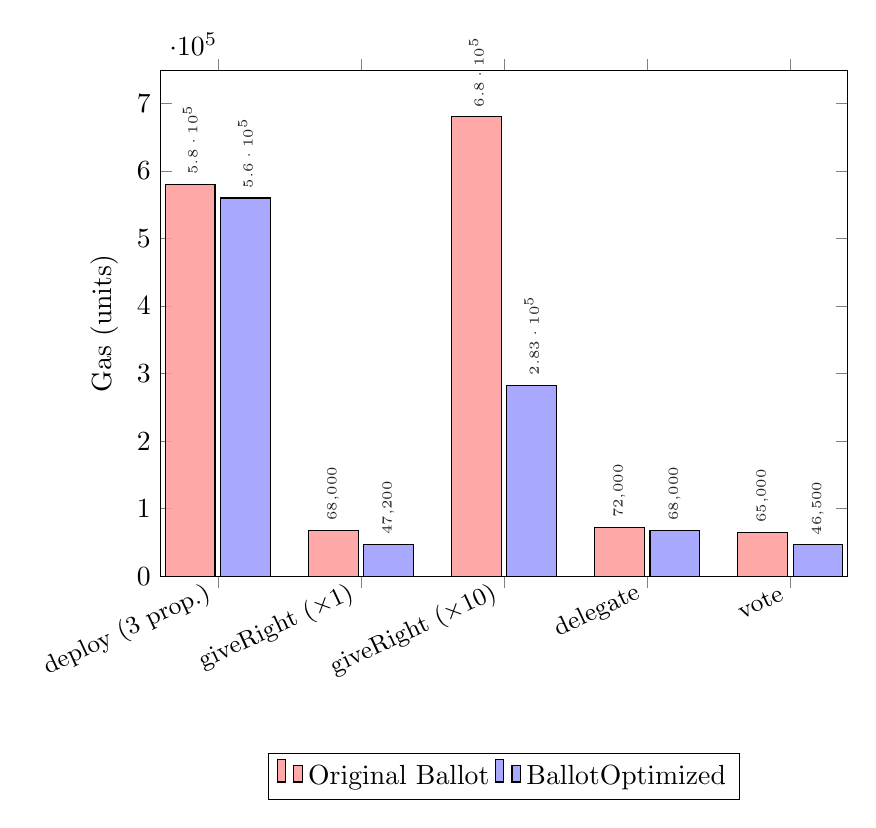
\begin{tikzpicture}
        \begin{axis}[
            ybar,
            bar width=18pt,
            width=0.85\textwidth,
            height=8cm,
            ylabel={Gas (units)},
            symbolic x coords={
                {deploy (3~prop.)},
                {giveRight ($\times$1)},
                {giveRight ($\times$10)},
                {delegate},
                {vote}
            },
            xtick=data,
            x tick label style={rotate=25, anchor=east, font=\small},
            ymin=0,
            legend style={at={(0.5,-0.35)}, anchor=north, legend columns=2},
            nodes near coords,
            nodes near coords style={font=\tiny, rotate=90, anchor=west},
            every axis plot/.append style={fill opacity=0.85},
        ]
            % Original (approximate values)
            \addplot[fill=red!40] coordinates {
                ({deploy (3~prop.)}, 580000)
                ({giveRight ($\times$1)}, 68000)
                ({giveRight ($\times$10)}, 680000)
                ({delegate}, 72000)
                ({vote}, 65000)
            };
            % Optimised (approximate values)
            \addplot[fill=blue!40] coordinates {
                ({deploy (3~prop.)}, 560000)
                ({giveRight ($\times$1)}, 47200)
                ({giveRight ($\times$10)}, 283000)
                ({delegate}, 68000)
                ({vote}, 46500)
            };
            \legend{Original Ballot, BallotOptimized}
        \end{axis}
    \end{tikzpicture}
    \caption{Approximate gas costs: original vs. optimised Ballot contract.}
    \label{fig:gas}
\end{figure}

Найбільш істотна економія гасу вже відчувається при наданні прав голосування 10 виборцям в рамках однієї пакетної транзакції.

\section{Розгортання контракту via Remix IDE}
\label{sec:deploy}

\subsection{Попередня підготовка}

\begin{itemize}
    \item Встановити та налаштовати розширення браузера MetaMask.
    \item Підключити MetaMask до тестової мережі \textbf{Sepolia}.
    \item Накопичити трохи SepoliaETH у гаманці, наприклад з крану \href{https://cloud.google.com/application/web3/faucet/ethereum/sepolia}{CloudGoogle}.
    \item Залогінитися на Remix~\cite{remix-ide} і SepoliaEtherscan~\cite{sepolia-etherscan}.
\end{itemize}

\subsection{Інструкція з деплойменту}

\begin{enumerate}[label=\textbf{\arabic*.}, leftmargin=2em]
    \item \textbf{Open Remix IDE} at \url{https://remix.ethereum.org}.
    \item \textbf{Create the contract file.} В панельці зліва (File Explorer), у папці contracts створюємо новий файл з 
    назвою: \texttt{BallotOptimized.sol}. Копіпастимо оптимізований код контракту з розділу~\ref{sec:gasopt}.
    \item \textbf{Configure the compiler.} Переходимо на вкладку "Solidity Compiler"{} (третя піктограма в лівій бічній панелі). 
        Встановлюємо версію компілятора \texttt{0.8.21} (або будь-яку сумісну версію 0.8.x). Також ставимо галочку 
        біля \emph{Enable optimization} і вводимо кількість запусків --- \texttt{200}. Натисніть \textbf{Compile BallotOptimized.sol}. 
        Очікуємо на зелену галочку.
    \begin{figure}[H]
        \centering
        \includegraphics[width=0.85\textwidth]{screenshots/screen1.png}
        \caption{Remix IDE: Compiler settings for BallotOptimized.sol.}
        \label{fig:screen1}
    \end{figure}
    \item \textbf{Connect MetaMask.} Змінюємо вкладинку на Deploy \& Run Transactions.  У розділі \textbf{Environment} 
        вибираємо \texttt{WalletConnect MetaMask}. Підтверджуємо зв'язок. Перевіряємо, що в MetaMask вибрана Sepolia, а адреса нашого 
            облікового запису відображається в Remix.
    \item \textbf{Prepare constructor arguments.} Конструктор очікує від нас \texttt{bytes32[]} --- масив імен пропозицій, закодованих у 
        вигляді 32-байтових шістнадцяткових рядків. Підготуйте їх за допомогою консолі Remix або вручну:
        \begin{code}
            // In Remix console (bottom panel):
            web3.utils.asciiToHex("OptionA")
            // Result: 0x4f7074696f6e41000000...00
            // Deploy input field format:
            ["0x4f7074696f6e4100...", "0x4f7074696f6e4200...",
            "0x4f7074696f6e4300..."]
        \end{code}
    \item \textbf{Deploy.} Вставляємо масив \texttt{bytes32[]} у поле введення і тиснемо кнопку "transact". 
        Підтверджуємо транзакцію в MetaMask. Чекаємо 15-30 секунд, поки Sepolia вибудує блок з нашим контрактом.
        \begin{figure}[H]
            \centering
            \includegraphics[width=0.7\textwidth]{screenshots/screen2.png}
            \caption{MetaMask transaction confirmation.}
            \label{fig:screen2}
        \end{figure}
    \item \textbf{Interact with the contract.} Розгорнутий контракт з'являється в розділі "Deployed Contracts"{} внизу, на тій же панелі. 
        Потестимо наступні функції:
        \begin{enumerate}[label=\alph*), leftmargin=1.5em]
            \item Тиснемо \texttt{chairperson} --- з'являєтсья наша адреса, з якої деплоїли контракт.
            \item Викликаємо \texttt{giveRightToVote} з адресою другого облікового запису MetaMask.
            \item Перемикаємо обліковий запис, і викликаємо \texttt{vote(0)}.
            \item Викликаємо \texttt{winnerName()} --- і бачимо, що повертається \texttt{bytes32} наш "OptionA"{}.
        \end{enumerate}
        \begin{figure}[H]
            \centering
            \begin{minipage}{0.45\textwidth}
                \centering
                \includegraphics[width=\textwidth]{screenshots/screen3.png}
                \caption{Deployed contract panel with function results.}
                \label{fig:screen3}
            \end{minipage}
            \hfill
            \begin{minipage}{0.5\textwidth}
                \centering
                \includegraphics[width=\textwidth]{screenshots/screen4.png}
                \caption{Second account providing voting rights and casting a vote.}
                \label{fig:screen4}
            \end{minipage}
        \end{figure}
    \item \textbf{Verify on Etherscan.} Переглянемо наш контакт і виконані (оранжеві) транзакції на Etherscan: \\ 
        \texttt{https://sepolia.etherscan.io/address/<CONTRACT\_ADDRESS>}.\\
        Тут можемо спостерігати всі транзакції, включаючи розгортання та виклики функцій. Клікнувши на кожну транзакцію, ми 
        можемо побачити деталі, включаючи витрати газу.
        \begin{figure}[H]
            \centering
            \includegraphics[width=0.85\textwidth]{screenshots/screen5.png}
            \caption{Etherscan transaction list for the deployed BallotOptimized contract.}
            \label{fig:screen5}
        \end{figure}
\end{enumerate}

Для зручності, ось ще таблиця з прикладами застосованих імен пропозицій та їх \texttt{bytes32} представленнями:

\begin{tblr}{
    colspec = {Q[l, m, 70pt]Q[l, m, font=\footnotesize\ttfamily]},
    row{1} = {font=\bfseries\small, bg=gray!15, c},
    hlines, vlines,
    width = \textwidth,
    measure = vbox,
}
    Proposal Name & {bytes32 Hex Value} \\
    OptionA & 0x4f7074696f6e4100000000000000000000000000000000000000000000000000 \\
    OptionB & 0x4f7074696f6e4200000000000000000000000000000000000000000000000000 \\
    OptionC & 0x4f7074696f6e4300000000000000000000000000000000000000000000000000 \\
\end{tblr}

\section{Висновки для завдання~1}

В цій частині я:
\begin{enumerate}
    \item Розглянув, як працюють смарт-контракти Ethereum на загальному рівні (життєвий цикл, модель зберігання, механізм використання 
        газу).
    \item Обрав контракт \textbf{Ballot (Voting)} з документації Solidity 0.5.3 як найбільш suitable приклад для цієї 
        лабораторної роботи та розглянув детально, проаналізувавши його структури даних, змінні станів та функції.
    \item Разом з ШІ (куди без нього) зробили оптимізовану версію (\texttt{BallotOptimized.sol}) з 8 моментами покращення в економії газу: 
        включаючи batch реєстрацію виборців, \texttt{external} видимість, \texttt{unchecked} арифметику, обмеження ланцюжка делегування та 
        оптимізацію циклів.
    \item Розгорнув оптимізований контракт у тестовій мережі Sepolia за допомогою Remix IDE та MetaMask і повчився розгортати контракт, 
    а також взаємодіяти з ним, перевіряючи транзакції на Sepolia Etherscan.
\end{enumerate}
